\subsection*{Problema y modelo}

El problema consiste en encontrar el camino para que Alice visite caminando
a Bob minimizando la cantidad de subidas y bajadas que debe atravesar. La
descripción del terreno consiste en un mapa de alturas, compuesto por
polígonos que no se intersecan entre sí ni consigo mismos. Cada polígono
informa la altura del terreno sobre su perímetro.

La descripción que nos dan del terreno es parcial, pues no sabemos qué
alturas hay en el terreno en medio de cualquier par de curvas de altura
distintas. Por ello no podemos saber exactamente cuánto escala o desciende
Alice en su camino, pero podemos calcular el mínimo suponiendo un escenario
óptimo.

Presentamos un modelo simple en el que representamos los polígonos como
un conjunto de segmentos en los ejes $X\ Y$. Cada segmento tiene un valor de
altura dado por el enunciado. Alice y Bob se encuentran en las coordenadas
dadas por el enunciado (Alice en $(0,0)$, y Bob en $(100.000,0)$).

\subsection*{Solución}

Nuestra solución se basa en las siguientes ideas:

\begin{itemize}
\item Dado que no existe intersección entre polígonos, para cualquier par de
polígonos ocurre uno contiene al otro, o que son completamente disjuntos.

\item Distinguimos los polígonos según si Alice tiene que cruzarlos
obligatoriamente, o si puede evitarlos. De esta forma, ella cruza solamente
aquellos que necesariamente tiene que cruzar para ver a Bob. Un polígono es
evitable si existe algún camino entre las dos personas que no lo cruza.

\item Dado que no se puede saber cuáles son las alturas del terreno que
se ubica entre dos curvas de altura de distintos polígonos, la altura del
perímetro de cada polígono es independiente de la de los demás.
\end{itemize}

Cada vez que Alice cruza un polígono, la altura que debe escalar/bajar aumenta,
lo que significa que estos valores dependen de la cantidad y el orden de los
polígonos que cruza Alice. Logramos una cantidad mínima de polígonos cruzados si
respetamos el segundo principio.

Clasificar todos los polígonos según:

\begin{itemize}
\item Contiene solamente a Alice: para llegar a Bob, Alice va a tener que
cruzarlo, por lo que estos polígonos no son evitables.

\item Contiene solamente a Bob: Alice está fuera de este polígono, y necesita
cruzarlo, pues sino no podrá cumplir su objetivo. Estos polígonos no son
evitables.

\item No contiene a Alice ni a Bob: este polígono es evitable, es decir,
Alice no necesita cruzarlo para llegar a Bob, pues suponiendo que ella lo cruza
debe entrar y luego salir; llegaría a algún lugar al que le era posible llegar 
rodeando el polígono en cuestión sin necesidad de cruzarlo.

\item Contiene a ambos: Alice se puede mantener dentro de este polígono
y no necesita cruzarlo, de modo que también es evitable. En caso de que
Alice salga de este polígono, luego para llegar a Bob deberá cruzarlo. Si
consideramos el estado incial de Alice (justo antes de cruzar este polígono)
y su estado final (justo después de cruzarlo nuevamente) podemos decir que
siempre existe un camino entre estos estados inicial y final que no lo cruza
nunca ni atraviesa otros polígonos.
\end{itemize}

La solución al problema presentada ignora completamente los polígonos
evitables, dado que la altura de un polígono es independiente de la de los
demás. Consideremos entonces los polígonos no evitables.

Notemos que se puede definir un orden total entre los polígonos que contienen
solamente a Alice, y otro para los que contienen solamente a Bob. Consideramos
ordenado a una secuencia de polígonos tal que el primero es contenido por
todos los siguientes, y el último contiene a todos los anteriores. Esto
nos permite afirmar que existe una única solución para cada escenario del
problema, pues hay una sola forma de cruzar los polígonos que contienen a
Alice (de ``adentro'' hacia ``afuera''), y una sola forma de cruzar los que
contienen a Bob (de ``afuera'' hacia ``adentro''). Esta idea justifica la
solución presentada.

Dado un escenario, para cada polígono verificamos si contiene a Alice y
no a Bob o si contiene a Bob y no a Alice (ver sección ``Determinación
de pertenencia de un punto a un polígono''). En estos casos traducimos
el polígono a un par $(x_1, x_2, h)$ tal que $x_1$ y $x_2$ son dos puntos
distintos de intersección con el eje X, $x_1$ está a la izquierda del punto
que verificamos, $x_2$ a la derecha, y $h$ es la altura de las curvas de altura
del polígono. Podemos abstraernos de esta forma gracias a que los polígonos
están contenidos o totalmente disjuntos, de modo que para definir un orden
total entre los que están contenidos es suficiente con conocer cualquier par de
puntos de sus perímetros. En particular, nosotros tomamos la intersección
con el eje $X$ para describir los polígonos dado que debemos usar estos
puntos previamente para verificar la pertenencia de Alice (o de Bob).

Separamos en dos secuencias los pares que representan los polígonos que
cumplen que contienen a Alice y no a Bob, o que contienen a Bob y no a Alice. A
continuación ordenamos estas secuencias por contención de intervalos
(según la idea explicada en el párrafo anterior).

Luego recorremos de principio a fin la secuencia de pares que representan los
polígonos que contienen solamente a Alice, sumando en acumuladores de altura
escalada y altura bajada según corresponda. Lo recorremos en este orden
porque, para que Alice pueda salir de todos estos polígonos, primero tiene que
cruzar el más contenido y por último el que contiene a todos. Procedemos
análogamente para la secuencia de pares que representan los polígonos que
contienen sólo a Bob, pero recorriéndola de fin a principio. Lo recorremos
en este orden porque para que Alice pueda llegar a Bob debe cruzar primero el
polígono que contiene a todos, y por último el que es contenido por todos
(que es donde está Bob).

Finalmente devolvemos como resultado los acumuladores en el orden pedido
por el enunciado: primero la cantidad escalada, y luego la cantidad bajada.

\subsection*{Determinación de pertenencia de un punto a un polígono}

Para determinar si un punto está dentro de un polígono la solución utilizada es trazar una recta horizontal
que pase por el punto y verificar la intersección de esta recta con los lados del polígono. Esto implica
que necesitamos calcular la intersección entre una recta y un segmento.
Haciendo esto con todos los segmentos del polígono, guardamos la cantidad de cruces a izquierda del punto
en cuestión. Si la cantidad de cruces es impar, entonces el punto cae sobre el polígono, sino no (visto en
clase). Intuitivamente en cada cruce impar el polígono se está abriendo, y en cada cruce par se está
cerrando el sector abierto en el cruce impar inmediatamente anterior.
En particular, en nuestro problema la recta es el eje X, y los segmentos $<(x_1, y_1), (x_2, y_2)>$ son
los lados del polígono. Si cumple la condición de existencia de intersección (que explicaremos luego)
debemos resolver el sistema:

\vspace{0.2cm}
$(x_1, y_1) + \beta(x_2 - x_1, y_2 - y_1) = (x, 0)$
\vspace{0.2cm}

Despejando nos queda:

\vspace{0.2cm}
$\beta = -\displaystyle\frac{y_1}{y_2 - y_1}$
\vspace{0.2cm}

Y reemplazando, el resultado es:

\vspace{0.2cm}
$x = x_1 -\displaystyle\frac{(x_2 - x_1)y_1}{(y_2 - y_1)}$
\vspace{0.2cm}

Y tenemos la coordenada x de la intersección.

La condición de existencia de intersección verifica si:

\vspace{0.2cm}
$( y_1 < 0 \wedge y_2 \ge 0 ) \vee ( y_1 \ge 0 \wedge y_2 < 0 )$
\vspace{0.2cm}

Es evidente que si $( y_1 < 0 \wedge y_2 > 0 ) \vee ( y_1 > 0 \wedge y_2 < 0 )$ hay una intersección, pero si un
extremo del segmento cae sobre la recta debemos considerar casos especiales o arreglarlo de algún modo.

La forma de arreglarlo es simple pero requiere ser explicada con detenimiento. La idea es que si algun
extremo del segmento cae sobre la recta, si el otro extremo del segmento está arriba de la recta, entonces
contamos el cruce, sino no. Este particular método no verifica intersecciones entre cualquier recta y
cualquier segmento, pero sí nos sirve para el problema de verificar si un punto cae dentro de un polígono.

Los casos especiales que se pueden presentar en el cálculo de intersecciones de una recta con un polígono
que no se cruza consigo mismo son los siguientes:

\begin{itemize}

\begin{figure}[H]
\centering
\label{w_1}
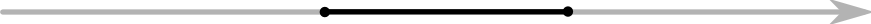
\includegraphics[scale=1.0]{./figuras/w_1.png}
\end{figure}

\item un segmento del polígono es paralelo a la recta y cae sobre ella, de modo que la intersección entre
ellos tiene infinitas soluciones. Este caso no pasa la condición que vimos, por lo que no genera
intersecciones. Intuitivamente, un segmento horizontal no cierra ni abre al polígono.

\item un vértice del polígono cae sobre la recta. Hay 4 tipos casos de estos:

\begin{figure}[H]
\centering
\label{w_2y3}
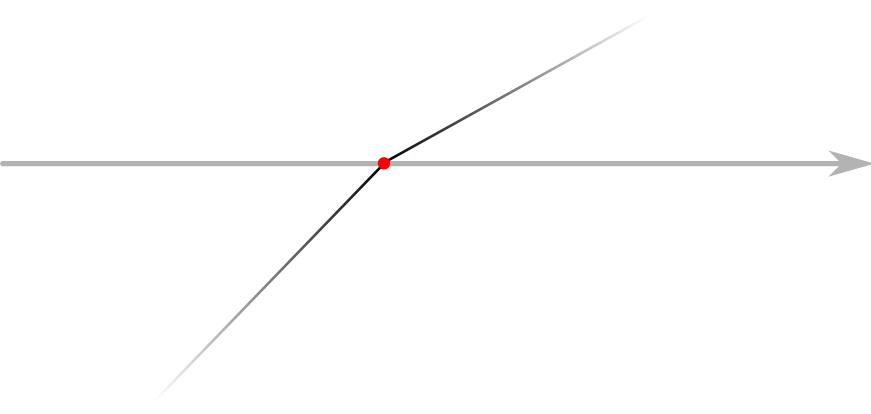
\includegraphics[scale=0.8]{./figuras/w_2.png}
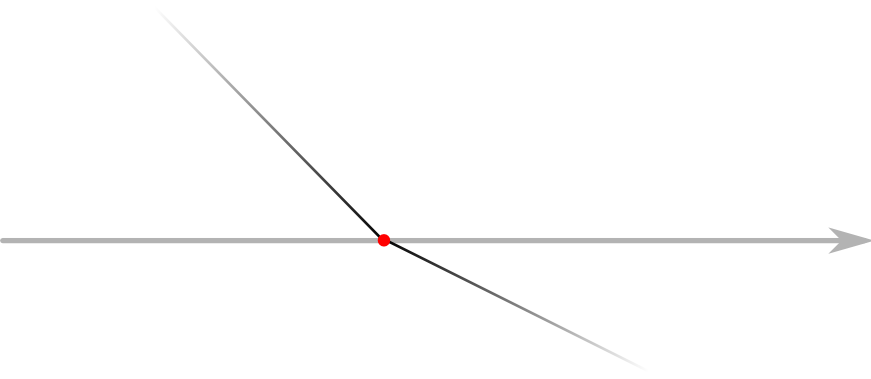
\includegraphics[scale=0.8]{./figuras/w_3.png}
\end{figure}

Intuitivamente, estos casos abren (primer figura) o cierran (segunda figura) el polígono, por lo que debe
contarse un cruce naturalmente, igual que los casos comunes en los que un segmento cruza la recta.

\begin{figure}[H]
\centering
\label{w_4y5}
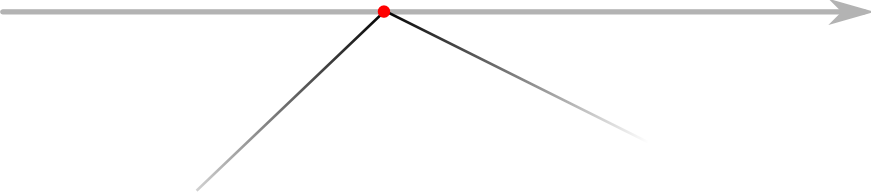
\includegraphics[scale=0.8]{./figuras/w_4.png}
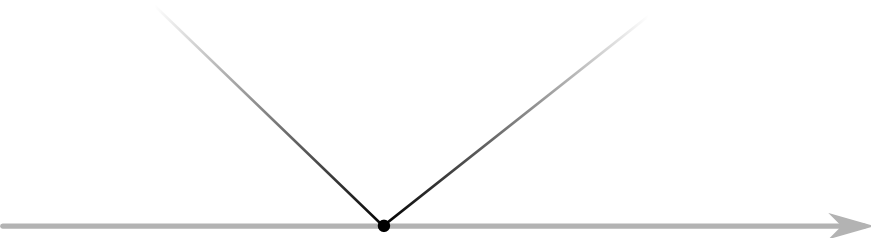
\includegraphics[scale=0.8]{./figuras/w_5.png}
\end{figure}

Intuitivamente, estos casos cierran y vuelven a abrir el polígono, por lo que debe mantener la paridad de
la cantidad de cruces. Si los lados del polígono que tienen este vértice como extremo tienen el otro extremo
por encima de la recta, la cantidad de cruces contados son 2 (uno por cada segmento), por lo que la paridad se
mantiene. Si los lados tienen el otro extremo por debajo de la recta, no se cuentan cruces (pues no cumple con
la condición).
\end{itemize}

\subsection*{Detalles de Implementación}

Se implementó la clase \textbf{Desnivel} que representa los polígonos según su cruce con el eje $X$.
Contiene dos números reales $x_1$, $x_2$ y un entero $altura$, que es la altura de las curvas de altura
del polígono.

Se implementó un método \textbf{contenido}, que dados dos Desniveles $a$ y $b$ verifica si
$b.x1 < a.x1 \wedge a.x2 < b.x2$.

El conjunto de polígonos que contienen solamente a Alice y el de polígonos que contienen solamente a Bob
se implementaron con dos vector de desniveles (uno para cada uno). El método de ordenamiento de estos
vectores es $Quicksort$ y utiliza como condición el método \textbf{contenido}.

\subsection*{Pseudocódigo}

\begin{algorithm}[H]
\linesnumbered
\caption{walk($poligonos$)}
\Input{polígonos que forman las curvas de nivel del escenario}
\vspace{0.4cm}
\For{cada polígono} {
    \For{cada lado del polígono} {
        \If{cumple la condición de cruce con el eje $X$} {
            \If{el cruce es a la izq de Alice} {
                $cruceIzqAlice \gets$ cruce del segmento con el eje $X$
                
                $crucesIzqAlice++$
            }
            \If{el cruce es en el medio de Alice y Bob} {
                $cruceDerAlice \gets$ cruce del segmento con el eje $X$
                
                $cruceIzqBob \gets$ cruce del segmento con el eje $X$
                
                $crucesMedio++$
            }
            \If{el cruce es a la derecha de Bob} {
                $cruceDerBob \gets$ cruce del segmento con el eje $X$
            }
        }
    }
    
    \If{el polígono contiene a Alice y no a Bob} {
        $poligonosAlice \gets$ agregar $<cruceIzqAlice, cruceDerAlice, poligono.altura>$
    }
    \If{el polígono contiene a Bob y no a Alice} {
        $poligonosBob \gets$ agregar $<cruceIzqBob, cruceDerBob, poligono.altura>$
    }
}

calcularAlturaSubidaYBajada( poligonosAlice, poligonosBob )
\end{algorithm}

\begin{algorithm}[H]
\linesnumbered
\caption{calcularAlturaSubidaYBajada($poligonosAlice, poligonosBob$)}
\Input{vectores de pares que representan los poligonos que contienen solamente a Alice y los que contienen
solamente a Bob}
\vspace{0.4cm}

ordenar las secuencias poligonosAlice y poligonosBob por contención

$alturaSubida \gets 0$

$alturaBajada \gets 0$

\If{existe algún polígono que contenga a Alice} {
    $ultimaAltura \gets$ altura de $poligonosAlice.primero$
    
    \For{cada par $p$ en poligonosAlice despues del primero} {
        \If{$p.h < ultimaAltura$} {
            $alturaBajada \gets alturaBajada + ultimaAltura - p.h$
        }
        \Else {
            $alturaSubida \gets p.h - ultimaAltura$
        }
        
        $ultimaAltura \gets p.h$
    }
}

\If{existe algún polígono que contenga a Bob} {
    \If{no existe polígono que contenga a Alice} {
        $ultimaAltura \gets$ altura de $poligonosBob.primero$
        
        $poligonosBob \gets$ sacar primer elemento de la secuencia
    }
    
    \For{cada par $p$ en poligonosBob desde el último al primero} {
        \If{$p.h < ultimaAltura$} {
            $alturaBajada \gets alturaBajada + ultimaAltura - p.h$
        }
        \Else {
            $alturaSubida \gets p.h - ultimaAltura$
        }
        
        $ultimaAltura \gets p.h$
    }
}

imprimir alturaSubida alturaBajada
\end{algorithm}

\subsection*{Análisis de complejidad}
A continuación se analizará la complejidad del algoritmo walk que soluciona del problema.

\textbf{calcularAlturaSubidaYBajada:}

La primer línea realiza un ordenamiento de dos vectores. En peor caso esta línea tiene complejidad
$O(max(a,b)^2)$, siendo $a$ la cantidad de elementos del vector poligonosAlice, y $b$ la cantidad de
elementos del vector polígonosBob. El caso promedio de esta línea es $O(max(a,b)*log(max(a,b)))$

Las líneas 2 hasta la 5 tienen costo constante, pues se trata de consultas y asignaciones a variables
resolubles en tiempo constante, al igual que el cuerpo del ciclo de la línea 6.

El ciclo de la línea 6 se ejecuta a lo sumo $a - 1$ veces, por lo tanto las líneas de 4 a 15 tienen
complejidad $O(a)$.

Las líneas 16 hasta la 20 tienen costo constante, pues se trata de consultas y asignaciones a variables
resolubles en tiempo constante, al igual que el cuerpo del ciclo de la línea 21.

El ciclo de la línea 21 se ejecuta a lo sumo $b - 1$ veces, por lo tanto las líneas de 16 a 30 tienen
complejidad $O(b)$.

La línea 31 tiene complejidad constante.

Por lo tanto el algoritmo completo calcularAlturaSubidaYBajada tiene complejidad $O(max(a,b)^2)$ en
peor caso, y $O(max(a,b)*log(max(a,b)))$ en caso promedio, siendo $a$ y $b$ los que dijimos
anteriormente.

\textbf{walk:}

Las líneas 3 hasta la 16 tienen costo constante, pues se trata de consultas y asignaciones a variables
resolubles en tiempo constante.

El ciclo de la línea 2 se ejecuta a lo sumo $P_i + 1$ veces, siendo $P_i$ la cantidad de vértices del
polígono $i$. Por lo tanto este ciclo tiene complejidad $O(P_i)$.

Las líneas desde la 18 hasta la 23 tienen costo constante, ya que se trata de consultas y pusheo de un
elemento al final de un vector.

El ciclo de la línea 1 se ejecuta a lo sumo $N$ veces, siendo $N$ la cantidad de polígonos.
Por lo tanto el ciclo completo (desde la línea 1 hasta la 24) tiene complejidad $O(N*max(P_i))$.

La línea 25 se trata de un llamado a calcularAlturaSubidaYBajada, lo que analizamos anteriormente, y
tiene complejidad $O(max(a,b)^2)$ en peor caso y $O(max(a,b)*log(max(a,b)))$ en caso promedio.
El peor caso en este problema para este algoritmo sería que todos los polígonos contengan a Alice o a Bob,
por lo que $max(a,b) = N$, y en caso promedio sería $max(a,b) = \frac{N}{2} +/- 1$ si es
par/impar, lo que hace la complejidad $O(N^2)$ en peor caso y $O(N*log(N))$ en caso promedio.

Por lo tanto el algoritmo completo walk tiene complejidad $O(N*max(P_i) + N^2)$ en peor caso,
y $O(N*max(P_i) + N*log(N))$ en caso promedio, siendo $N$ la cantidad de polígonos y
$P_i$ la cantidad de lados del polígono $i$.